\documentclass[11pt]{article}
\usepackage[utf8]{inputenc}
\usepackage[T1]{fontenc}
\usepackage[french]{babel}
\usepackage{amsmath}
\usepackage[bookmarks={true},bookmarksopen={true}]{hyperref}
\usepackage{graphicx}
\usepackage[a4paper]{geometry}
\usepackage{listings}
\usepackage{amssymb}
\usepackage{amsmath,amsfonts}
	\lstset{frame=tb,
		language=Java,
 		aboveskip=3mm,
  		belowskip=3mm,
  		showstringspaces=false,
  		columns=flexible,
  		basicstyle={\small\ttfamily},
  		numbers=none,
 		numberstyle=\tiny\color{gray},
  		keywordstyle=\color{blue},
  		commentstyle=\color{dkgreen},
  		stringstyle=\color{mauve},
  		breaklines=true,
  		breakatwhitespace=true
  		tabsize=3
	}
\pagestyle{plain}
\setlength{\parindent}{5mm}
\usepackage{amsmath}
\usepackage{color}
\definecolor{dkgreen}{rgb}{0,0.6,0}
\definecolor{gray}{rgb}{0.5,0.5,0.5}
\definecolor{mauve}{rgb}{0.58,0,0.82}



\title{\textbf{Projet LSINF1121 -  Algorithmique et structures de données\\ - \\ Rapport intermédiaire Mission 5} \\ {\large Groupe 26}}
\author{Laurian \bsc{Detiffe} \\(6380-12-00)\and Sundeep \bsc{Dhillon} \\(6401-11-00)\and Alexis \bsc{Macq} \\ (5910-12-00) \and Xavier \bsc{Pérignon} \\ (8025-11-00)\and Thibaut \bsc{Piquard}\\(4634-13-00)\and Thomas \bsc{Wyckmans} \\ (3601-12-00)}
\date{date}
\date{\vspace*{25mm}

\includegraphics[scale=0.75]{logo.jpg}\\
		\vspace*{30mm}
		\begin{center}
		Année académique 2015-2016 \\	
		\end{center}}

\begin{document}
\thispagestyle{empty}

\maketitle
\thispagestyle{empty}
%\tableofcontents
%\setcounter{tocdepth}{3}
%\setcounter{page}{1}
%\newpage

\section*{Questions et réponses}
\begin{enumerate}

\item
\item
\item
\item
\item
\item Quels sont les avantages et inconvénients éventuels d’implémenter une file de
priorité par un heap plutôt que par une liste ?
Existe-t-il un tas T mémorisant 7 éléments distincts tel qu’un parcours infixe du
tas renvoie les éléments de T en ordre décroissant ? Qu’en est-il avec un parcours
préfixe ou post-fixe ?

Les avantages sont une meilleure complexité calculatoire, 
($log(n)$ pour les opérations de recherches et n pour les insertions avec n le nombre d'éléments stockés),
une implémentation facile, un ordre partiel garanti. Les inconvénients sont une certaine
rigidité (utilisation d'un tableau), une efficacité qui implique une absence de
revérifications des propriétés du heap ce qui implique une grande vulnérabilité face à
d'éventuelles attaques et une insertion qui n'est pas plus rapide que dans une file de
priorités séquentielles.\\
Passons maintenant à la deuxième partie de la question : \\
Un binary heap respecte par définition la condition suivante : tous les noeuds qui sont plus proches de la racine qu'un certain noeud sont plus grand que celui-ci.
Soit le binary heap suivant,
$$ a[8] = {null, x_1, x_2, x_3, x_4, x_5, x_6, x_7} $$
qu'on peut représenter via l'arbre binaire suivant :\\
\begin{tikzpicture}
  \node{$x_1$}
   child {node {$x_2$}
           child {node {$x_4$}}
           child {node {$x_5$\ \ \ \ \ \ }}}
   child {node {$x_3$}
           child {node {\ \ \ \ \ \ $x_6$}}
           child {node {$x_7$}}};
\end{tikzpicture}\\
Un parcours infixe de ce binary heap nous donne la suite suivante :
$$ x_4 - x_2 - x_5 - x_1 - x_6 - x_3 - x_7 $$
Il est impossible que cet ordre de retour soit un ordre décroissant car cela impliquerait que $ x_4  > x_2 $ ce qui va en contradiction avec la définition d'un binary heap. \\
Un parcours préfixe de ce binary heap nous donne la suite suivante :
$$ x_1 - x_2 - x_4 - x_5 - x_3 - x_6 - x_7 $$
Cette ordre peut-être un ordre croissant sans violer la définition d'un binary heap. Par exemple : \\
\begin{tikzpicture}
  \node{$x_1 = 12$}
   child {node {$x_2 = 11$}
           child {node {$x_4 = 10$}}
           child {node {$9$\ \ \ \ \ \ }}}
   child {node {$x_3 = 8$}
           child {node {\ \ \ \ \ \ $7$}}
           child {node {$x_7 = 6$}}};
\end{tikzpicture}\\

Un parcours post-fixe de ce binary heap nous donne la suite suivante :
$$ x_4 - x_5 - x_2 - ... $$
Ce qui est impossible car la contrainte $ x_5 > x_2 $ viole la définition du binary heap.

\item
\item
\item

\item Quelles sont les différentes étapes d’un algorithme de compression de texte qui
prend en entrée un texte et fournit en sortie une version comprimée de ce texte à
l’aide d’un codage de Huffman ? Soyez précis dans votre description en isolant
chaque étape du problème. Précisez notamment pour chaque étape les structures
de données utiles et la complexité temporelle des opérations menées. (Xavier)\\

La méthode de Huffman consiste à remplacer les caractères les plus fréquents par des codes
courts et les caractères les moins fréquents par des codes longs. La phase d’encodage se compose de trois étapes :
\begin{enumerate}
\item \textbf{Comptage des fréquences des caractères} : cette étape consiste à parcourir tous les caractères du texte et à calculer le nombre d'occurence de chaque lettre dans ce texte. Si $n$ est le nombre de caractères dans le texte, alors la complexité de cette étape est de $O(n)$.
\begin{center}
    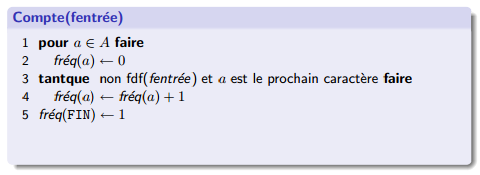
\includegraphics{comptage.PNG}
\end{center}
\item \textbf{Construction du code préfixe} : Un code préfixe est un ensemble de mots tel qu’aucun mot de
l’ensemble n’est préfixe d’un autre mot de l’ensemble. Un code préfixe sur l’alphabet binaire \{0, 1\} peut être représenté par
un tri qui est un fait un arbre binaire dont tous les nœuds internes ont exactement deux successeurs. Les feuilles sont étiquetées avec les caractères originaux, les branches par 0 ou 1 et les chemins depuis la racine jusqu’aux feuilles épellent les codes des caractères originaux. L’utilisation d’un code préfixe assure que les codes sont bien représentés par les feuilles. Par convention, le fils gauche d’un nœud est étiqueté par 0 et le fils droit
par 1.
\begin{center}
    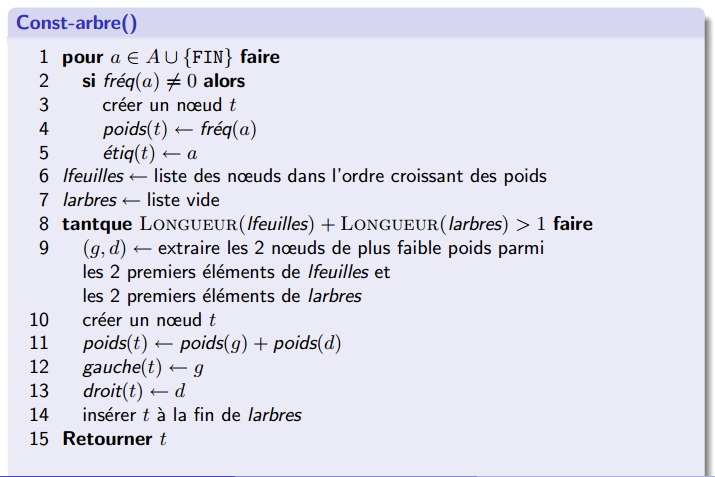
\includegraphics[scale=0.65]{arbre.PNG}
\end{center}
\item \textbf{Codage du texte} : Après la construction de l’arbre, il est possible de retrouver le code de
chaque caractère par un parcours en profondeur de l’arbre. 
\begin{center}
    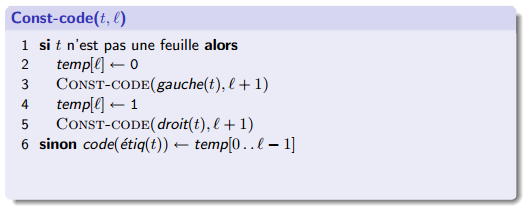
\includegraphics[scale=0.90]{constcode.PNG}
\end{center}
Cette étape nécessite de stocker les codes de chaque caractère avant le code du texte.
\begin{center}
    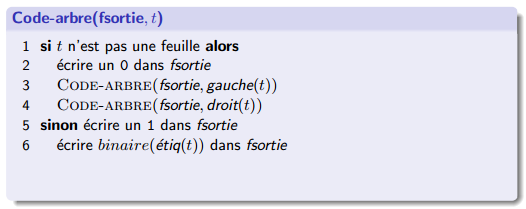
\includegraphics[scale=0.90]{codearbre.PNG}
\end{center}
On peut ensuite coder le texte.
\begin{center}
    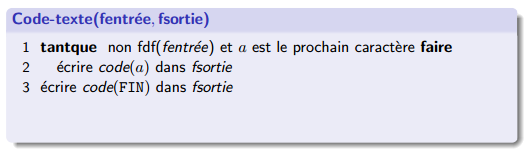
\includegraphics[scale=0.90]{codetexte.PNG}
\end{center}
La complexité de cette étape est le la complexité d'un parcours d'un arbre binaire, c'est-à-dire en $O(n log(n))$.\\
\end{enumerate}

\item

\item \textbf{[Question liée spécifiquement au problème posé]} En quoi les deux classes qui
vous sont fournies, \texttt{\textbf{InputBitStream}} et \texttt{\textbf{OutputBitStream}}, peuvent-elles
être utiles pour le problème de compression et de décompression avec un codage
de Huffman ? La postcondition de la méthode \texttt{\textit{close}} dans la classe \texttt{\textbf{OutputBitStream}}
précise notamment que \textit{si le nombre de bits déjà écrits ne correspond pas à un
multiple de 8 (un octet), des bits à 0 sont écrits pour compléter l’octet courant}.
Quand la situation décrite peut-elle se présenter ? Quelle est la conséquence de
cette postcondition sur votre programme de compression de texte ? Quelle est la
conséquence de cette postcondition sur votre programme de décompression ? (Xavier)\\

Les classes \texttt{\textbf{InputBitStream}} et \texttt{\textbf{OutputBitStream}} ont pour but de lire et d'écrire des bits, dont l'entrée et la sortie standard sont orientés vers les flux de caractères encodés en Unicode. La valeur d'un $int$ sur la sortie standard est une séquence de caractères (représentation décimale), tandis que la valeur d'un $int$ sur \texttt{\textbf{OutputBitStream}} est une séquence de bits (représentation binaire). Ces classes  fondent leur I/O sur 8-bit bytestreams. Les données sur l'entrée standard ne sont pas nécessairement alignés sur les frontières d'octets. La méthode \texttt{\textit{close}} n'est pas indispensable mais, pour une terminaison propre, les utilisateurs devraient appeler \texttt{\textit{close}} pour indiquer qu'il n'y a plus de bits à lire (pour la compression). Pour la décompression, la méthode \texttt{\textit{close}} est essentielle. En effet, les utilisateurs doivent appeler \texttt{\textit{close}} pour veiller à ce que tous les bits spécifiés avec les appels \texttt{\textit{write}} s'écrivent dans la $bitstream$ et que le dernier octet se remplisse avec des 0 afin que output s'aligne avec le système de fichiers.\\

\item
\item

\end{enumerate}
\end{document}